\documentclass{standalone}
\usepackage{tikz}
\usepackage{tikz-network}

\begin{document}
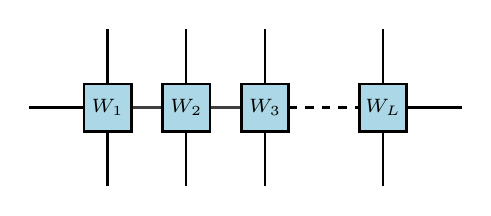
\begin{tikzpicture}
    % Main vertices (circles)
    \Vertex[x=0, y=0, label=$W_1$, shape=rectangle]{A}
    \Vertex[x=1, y=0, label=$W_2$, shape=rectangle]{B}
    \Vertex[x=2, y=0, label=$W_3$, shape=rectangle]{C}
    \Vertex[x=3.5, y=0, label=$W_L$, shape=rectangle]{D}

    % Horizontal edges
    \Edge[lw=1pt](A)(B)
    \Edge[lw=1pt](B)(C)
    \draw[dashed, thick] (C) -- (D);
    
    % Vertical legs (upward)
    \draw[thick] (A) -- (-1, 0);
    \draw[thick] (A) -- (0, 1);
    \draw[thick] (B) -- (1, 1);
    \draw[thick] (C) -- (2, 1);
    \draw[thick] (D) -- (3.5, 1);
    \draw[thick] (D) -- (4.5, 0);
    
    % Vertical legs (downward)
    \draw[thick] (A) -- (0, -1);
    \draw[thick] (B) -- (1, -1);
    \draw[thick] (C) -- (2, -1);
    \draw[thick] (D) -- (3.5, -1);
\end{tikzpicture}
\end{document}
